%! TeX program = lualatex
\documentclass{article}
\usepackage[left=4cm,right=3cm,top=3cm,bottom=3cm, marginpar=3cm]{geometry}
\setlength{\parindent}{0pt}

\usepackage{cprotect}
\usepackage{tikz}
\usetikzlibrary{math}

\usepackage{xcolor}

\usepackage{hyperref}
\hypersetup{
    pdftitle={Easy colorblind-safe typesetting: the colorblind package},
    pdfauthor={Simon Pfahler},
}
\usepackage{cleveref}

\usepackage{csquotes}
\usepackage[backend=biber, style=numeric-comp, seconds=true, sorting=none, subentry=true, doi=false, alldates=iso]{biblatex}
\renewcommand*{\entrysetpunct}{\\[5pt]}
\addbibresource{bib.bib}

\usepackage[Tol, OkabeIto]{colorblind}

\newcommand\colorblind{\textbf{colorblind} }

\reversemarginpar
\newcommand\marg[1]{\leavevmode\marginpar{\raggedleft #1}}
\newcommand\tbs{\textbackslash}

\title{Easy colorblind-safe typesetting:\\ the \colorblind package}
\author{Simon Pfahler}
\date{\today\\Version 0.1}


\begin{document}

\maketitle

\begin{abstract}
    This package provides the tools necessary for colorblind-safe typesetting in \LaTeX.
    It provides color schemes for any application, including qualitative, diverging and sequential schemes.
    Additionally, this package enables checking colorblind-safeness continuously during writing\footnote{This is still future work}.
    Therefore, colorblind-safeness is incorporated into the writing process, making it both less cumbersome and less error-prone.
\end{abstract}

\tableofcontents

\section{Quick introduction}
\cprotect\marg{\verb!Tol!\\\verb!OkabeIto!}%
The primary function of the \colorblind package is to provide a set of color schemes suitable for a wide variety of applications.
For this purpose, the color schemes by Tol~\cite{Tol}, as well as the famous Okabe Ito color palette~\cite{Ichihara_2008} are implemented.
They can be activated by the package options \verb!Tol! or \verb!OkabeIto!.

All colors provided start with a prefix indicating the scheme they belong to, followed by a number (main colors) or the word \verb!gray! (color reserved for bad data).%
\cprotect\footnote{%
    The spelling \verb!grey! is also implemented, because I can never remember which one a given package uses.
}
The prefix for the different color schemes can be found in \cref{sec:colors}.

\cprotect\marg{\verb!\drawScheme{...}!}%
The visualizations of color schemes given in this documentation are created with the command \verb!\drawScheme{...}!.
Only the prefix of a color scheme should be provided to the command, e.g.\ \verb!\drawScheme{T-Q-B}! to print the qualitative bright scheme by Tol, as can be seen in \cref{fig:T-Q-B}.


\section{Provided color schemes}\label{sec:colors}

\subsection{Paul Tol's color schemes}

\subsubsection{Qualitative color schemes}

\begin{figure}[ht]
    \centering
    \drawScheme{T-Q-B}
    \caption{Bright qualitative color scheme by Paul Tol~\cite{Tol}.}
    \label{fig:T-Q-B}
\end{figure}

\begin{figure}[ht]
    \centering
    \drawScheme{T-Q-HC}
    \caption{High-contrast qualitative color scheme by Paul Tol~\cite{Tol}.}
    \label{fig:T-Q-HC}
\end{figure}

\begin{figure}[ht]
    \centering
    \drawScheme{T-Q-V}
    \caption{Vibrant qualitative color scheme by Paul Tol~\cite{Tol}.}
    \label{fig:T-Q-V}
\end{figure}

\begin{figure}[ht]
    \centering
    \drawScheme{T-Q-M}
    \caption{Muted qualitative color scheme by Paul Tol~\cite{Tol}.}
    \label{fig:T-Q-M}
\end{figure}

\begin{figure}[ht]
    \centering
    \drawScheme{T-Q-MC}
    \caption{Medium-contrast qualitative color scheme by Paul Tol~\cite{Tol}.}
    \label{fig:T-Q-MC}
\end{figure}

\begin{figure}[ht]
    \centering
    \drawScheme{T-Q-PH}
    \caption{Pale qualitative color scheme by Paul Tol~\cite{Tol}, for highlighting only.}
    \label{fig:T-Q-PH}
\end{figure}

\begin{figure}[ht]
    \centering
    \drawScheme{T-Q-DT}
    \caption{Dark qualitative color scheme by Paul Tol~\cite{Tol}, for text color only.}
    \label{fig:T-Q-DT}
\end{figure}

\begin{figure}[ht]
    \centering
    \drawScheme{T-Q-L}
    \caption{Light qualitative color scheme by Paul Tol~\cite{Tol}.}
    \label{fig:T-Q-L}
\end{figure}

\subsubsection{Diverging color schemes}

\begin{figure}[ht]
    \centering
    \drawScheme{T-D-S}
    \caption{Sunset diverging color scheme by Paul Tol~\cite{Tol}.}
    \label{fig:T-D-S}
\end{figure}

\begin{figure}[ht]
    \centering
    \drawScheme{T-D-BR}
    \caption{BuRd diverging color scheme by Paul Tol~\cite{Tol}.}
    \label{fig:T-D-BR}
\end{figure}

\begin{figure}[ht]
    \centering
    \drawScheme{T-D-PG}
    \caption{PRGn diverging color scheme by Paul Tol~\cite{Tol}.}
    \label{fig:T-D-PG}
\end{figure}

\subsubsection{Sequential color schemes}

\begin{figure}[ht]
    \centering
    \drawScheme{T-S-YB}
    \caption{YlOrBr sequential color scheme by Paul Tol~\cite{Tol}.}
    \label{fig:T-S-YB}
\end{figure}

\begin{figure}[ht]
    \centering
    \drawScheme{T-S-DR}
    \caption{Discrete Rainbow sequential color scheme by Paul Tol~\cite{Tol}.}
    \label{fig:T-S-DR}
\end{figure}

\subsection{Okabe Ito qualitative color scheme}

\begin{figure}[ht]
    \centering
    \drawScheme{OI}
    \caption{Okabe Ito qualitative color scheme~\cite{Ichihara_2008}.}
    \label{fig:OI}
\end{figure}


\section{Experimental and work in progress}

\let\oldcolor\color

\newcommand\normalvision{%
    \protect\renewcommand\color[1]{\oldcolor{##1}}%
}

\newcommand\protanopia{%
    \protect\renewcommand\color[1]{%
        \extractcolorspecs{##1}{\modelspec}{\colorspec}%
        \tikzmath{
            \r = array({\colorspec},0);
            \g = array({\colorspec},1);
            \b = array({\colorspec},2);
            \rp = pow(0.06425 + 0.677*pow(\g, 2.2) + 0.2802*pow(\r, 2.2), 1./2.2);
            \gp = pow(0.06425 + 0.677*pow(\g, 2.2) + 0.2802*pow(\r, 2.2), 1./2.2);
            \bp = pow(0.06425 + 0.95724*pow(\b, 2.2) + 0.02138*pow(\g, 2.2) - 0.02138*pow(\r, 2.2), 1./2.2);
        }%
        \oldcolor[rgb]{\rp,\gp,\bp}%
    }%
}

\newcommand\deuteranopia{%
    \protect\renewcommand\color[1]{%
        \extractcolorspecs{##1}{\modelspec}{\colorspec}%
        \tikzmath{
            \r = array({\colorspec},0);
            \g = array({\colorspec},1);
            \b = array({\colorspec},2);
            \rp = pow(0.01194 + 0.8806*pow(\g, 2.2) + 0.1115*pow(\r, 2.2), 1./2.2);
            \gp = pow(0.01194 + 0.8806*pow(\g, 2.2) + 0.1115*pow(\r, 2.2), 1./2.2);
            \bp = pow(0.01194 + 0.992052*pow(\b, 2.2) - 0.003974*pow(\g, 2.2) + 0.003974*pow(\r, 2.2), 1./2.2);
        }%
        \oldcolor[rgb]{\rp,\gp,\bp}%
    }%
}

\begin{figure}[ht]
    \centering
    \begin{tikzpicture}
        \newcommand{\dx}{1}
        \newcommand{\dy}{-1.5}
        \newcommand{\radius}{0.7}

        % test for non rgb color models
        \definecolor{hsbtest1}{rgb}{0.266, 0.465, 0.664}
        \definecolor{hsbtest2}{hsb}{0.266, 0.468, 0.664}
        
        % Tol's bright qualitative color scheme
        \fill[T-Q-B1] (0,0) circle (\radius);
        \fill[T-Q-B2] (\dx,0) circle (\radius);
        \fill[T-Q-B3] (2*\dx,0) circle (\radius);
        \fill[T-Q-B4] (3*\dx,0) circle (\radius);
        \fill[T-Q-B5] (4*\dx,0) circle (\radius);
        \fill[T-Q-B6] (5*\dx,0) circle (\radius);
        \fill[T-Q-Bgrey] (6*\dx,0) circle (\radius);

        \fill[hsbtest1] (8*\dx,0) circle (\radius);
        \fill[hsbtest2] (9*\dx,0) circle (\radius);
        
        {
        \protanopia
        \fill[T-Q-B1, rounded corners=0.7*\radius cm]
            (0-\radius,\dy-0.7*\radius) rectangle ++(2*\radius, 1.4*\radius);
        \fill[T-Q-B2, rounded corners=0.7*\radius cm]
            (\dx-\radius,\dy-0.7*\radius) rectangle ++(2*\radius, 1.4*\radius);
        \fill[T-Q-B3, rounded corners=0.7*\radius cm]
            (2*\dx-\radius,\dy-0.7*\radius) rectangle ++(2*\radius, 1.4*\radius);
        \fill[T-Q-B4, rounded corners=0.7*\radius cm]
            (3*\dx-\radius,\dy-0.7*\radius) rectangle ++(2*\radius, 1.4*\radius);
        \fill[T-Q-B5, rounded corners=0.7*\radius cm]
            (4*\dx-\radius,\dy-0.7*\radius) rectangle ++(2*\radius, 1.4*\radius);
        \fill[T-Q-B6, rounded corners=0.7*\radius cm]
            (5*\dx-\radius,\dy-0.7*\radius) rectangle ++(2*\radius, 1.4*\radius);
        \fill[T-Q-Bgrey, rounded corners=0.7*\radius cm]
            (6*\dx-\radius,\dy-0.7*\radius) rectangle ++(2*\radius, 1.4*\radius);

        \fill[hsbtest1, rounded corners=0.7*\radius cm]
            (8*\dx-\radius,\dy-0.7*\radius) rectangle ++(2*\radius, 1.4*\radius);
        \fill[hsbtest2, rounded corners=0.7*\radius cm]
            (9*\dx-\radius,\dy-0.7*\radius) rectangle ++(2*\radius, 1.4*\radius);

        }
        
        {
        \deuteranopia
        \fill[T-Q-B1, rounded corners=0.7*\radius cm]
            (0-\radius,1.8*\dy-0.7*\radius) rectangle ++(2*\radius, 1.4*\radius);
        \fill[T-Q-B2, rounded corners=0.7*\radius cm]
            (\dx-\radius,1.8*\dy-0.7*\radius) rectangle ++(2*\radius, 1.4*\radius);
        \fill[T-Q-B3, rounded corners=0.7*\radius cm]
            (2*\dx-\radius,1.8*\dy-0.7*\radius) rectangle ++(2*\radius, 1.4*\radius);
        \fill[T-Q-B4, rounded corners=0.7*\radius cm]
            (3*\dx-\radius,1.8*\dy-0.7*\radius) rectangle ++(2*\radius, 1.4*\radius);
        \fill[T-Q-B5, rounded corners=0.7*\radius cm]
            (4*\dx-\radius,1.8*\dy-0.7*\radius) rectangle ++(2*\radius, 1.4*\radius);
        \fill[T-Q-B6, rounded corners=0.7*\radius cm]
            (5*\dx-\radius,1.8*\dy-0.7*\radius) rectangle ++(2*\radius, 1.4*\radius);
        \fill[T-Q-Bgrey, rounded corners=0.7*\radius cm]
            (6*\dx-\radius,1.8*\dy-0.7*\radius) rectangle ++(2*\radius, 1.4*\radius);
        
        \fill[hsbtest1, rounded corners=0.7*\radius cm]
            (8*\dx-\radius,1.8*\dy-0.7*\radius) rectangle ++(2*\radius, 1.4*\radius);
        \fill[hsbtest2, rounded corners=0.7*\radius cm]
            (9*\dx-\radius,1.8*\dy-0.7*\radius) rectangle ++(2*\radius, 1.4*\radius);
        }
    \end{tikzpicture}
    \caption{Test for deuteranopia and tritanopia commands: Left shows Tol's bright qualitative scheme, with deuteranopia and tritanopia vision in the second and third row. Right shows two colors with the same numbers in rgb and hsb, where the hsb variant gets translated incorrectly to color-deficient visions.}
\end{figure}

\begin{figure}[ht]
    \centering
    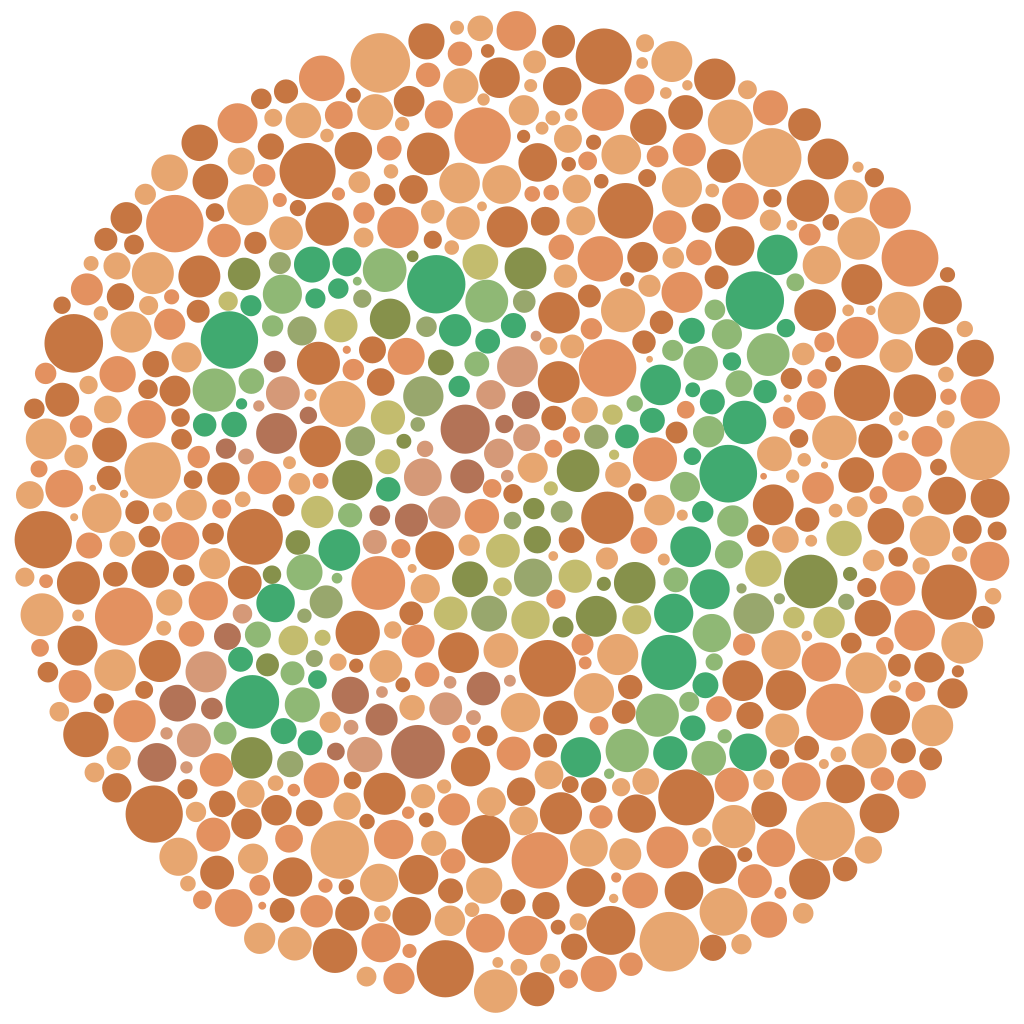
\includegraphics[width=0.3\textwidth]{Ishihara_9.png}
    \hspace{1cm}
    {\selectcolormodel{gray}
        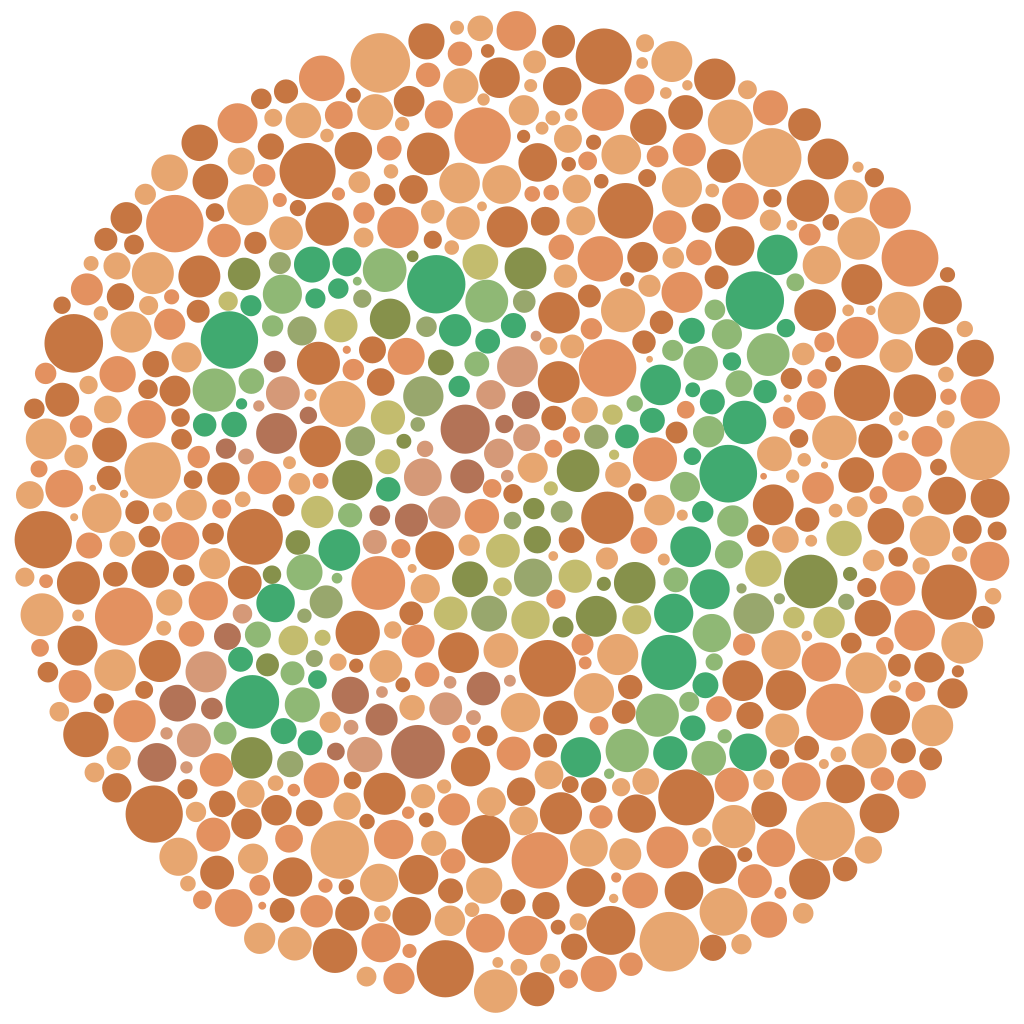
\includegraphics[decodearray={0 0 0 1 0 1}, width=0.3\textwidth]{Ishihara_9.png}
    }
    \caption{Ishihara colorblindness test, normal vision and without the {\color{red}red} channel.}
\end{figure}

\printbibliography

\end{document}
